\subsection{Graphs test}

\begin{figure}[h]
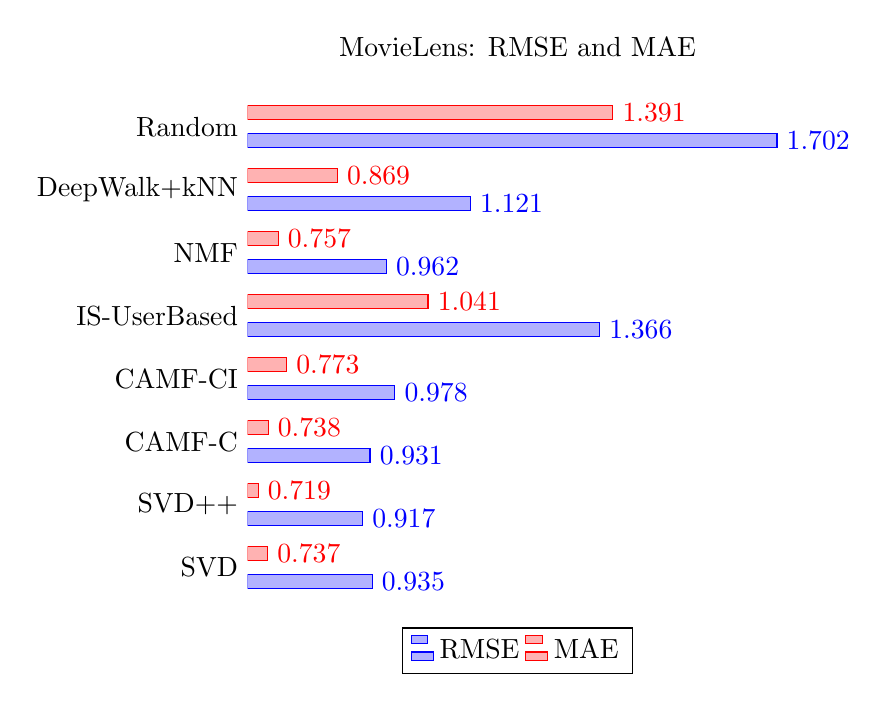
\begin{tikzpicture}
\begin{axis} [
    title    = {MovieLens: RMSE and MAE},
    xbar=5pt,
    /pgf/bar width=5pt,
    y axis line style = { opacity = 0 },
    axis x line       = none,
    tickwidth         = 0pt,
    enlarge x limits  = 0.02,
    ytick=data,
    y=0.8cm,
    nodes near coords={\pgfmathprintnumber[fixed zerofill, precision=3]{\pgfplotspointmeta}},
    legend style={at={(0.5,-0.03)}, anchor=north,legend columns=-1},
    symbolic y coords = {SVD,SVD++,CAMF-C,CAMF-CI,IS-UserBased,NMF,DeepWalk+kNN,Random},
  ]
\addplot coordinates{(0.935,SVD) (0.917,SVD++) (0.931,CAMF-C) (0.978,CAMF-CI) (1.366,IS-UserBased) (0.962,NMF) (1.121,DeepWalk+kNN) (1.702,Random)};
\addplot coordinates{(0.737,SVD) (0.719,SVD++) (0.738,CAMF-C) (0.773,CAMF-CI) (1.041,IS-UserBased) (0.757,NMF) (0.869,DeepWalk+kNN) (1.391,Random)};
\legend{RMSE,MAE}
\end{axis}
\end{tikzpicture}
\label{graph:MLRMSEMAE}
\caption{RMSE and MAE results for MovieLens dataset across the investigated methods}
\end{figure}

\begin{figure}[h]
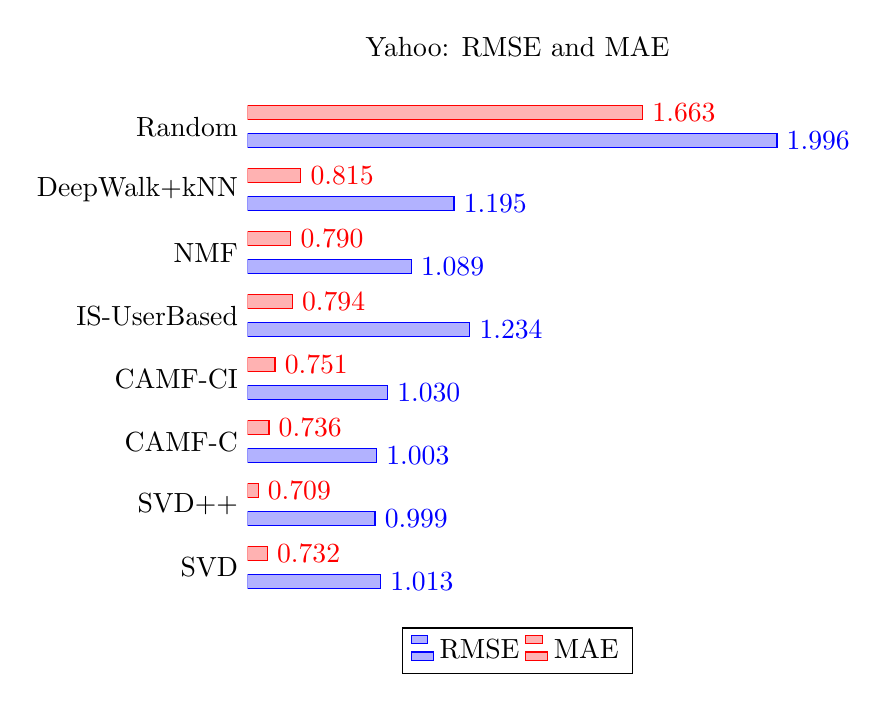
\begin{tikzpicture}
\begin{axis} [
    title    = {Yahoo: RMSE and MAE},
    xbar=5pt,
    /pgf/bar width=5pt,
    y axis line style = { opacity = 0 },
    axis x line       = none,
    tickwidth         = 0pt,
    enlarge x limits  = 0.02,
    ytick=data,
    y=0.8cm,
    nodes near coords={\pgfmathprintnumber[fixed zerofill, precision=3]{\pgfplotspointmeta}},
    legend style={at={(0.5,-0.03)}, anchor=north,legend columns=-1},
    symbolic y coords = {SVD,SVD++,CAMF-C,CAMF-CI,IS-UserBased,NMF,DeepWalk+kNN,Random},
  ]
\addplot coordinates{(1.013,SVD) (0.999,SVD++) (1.003,CAMF-C) (1.030,CAMF-CI) (1.234,IS-UserBased) (1.089,NMF) (1.195,DeepWalk+kNN) (1.996,Random)};
\addplot coordinates{(0.732,SVD) (0.709,SVD++) (0.736,CAMF-C) (0.751,CAMF-CI) (0.794,IS-UserBased) (0.790,NMF) (0.815,DeepWalk+kNN) (1.663,Random)};
\legend{RMSE,MAE}
\end{axis}
\end{tikzpicture}
\label{graph:YahooRMSEMAE}
\caption{RMSE and MAE results for Yahoo dataset across the investigated methods}
\end{figure}

\begin{figure}[h]
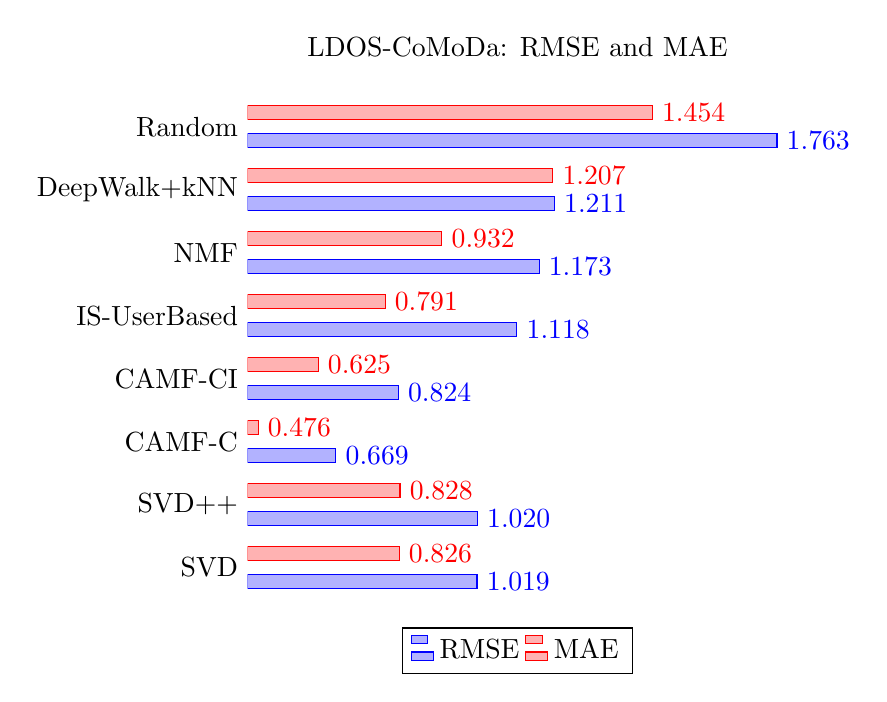
\begin{tikzpicture}
\begin{axis} [
    title    = {LDOS-CoMoDa: RMSE and MAE},
    xbar=5pt,
    /pgf/bar width=5pt,
    y axis line style = { opacity = 0 },
    axis x line       = none,
    tickwidth         = 0pt,
    enlarge x limits  = 0.02,
    ytick=data,
    y=0.8cm,
    nodes near coords={\pgfmathprintnumber[fixed zerofill, precision=3]{\pgfplotspointmeta}},
    legend style={at={(0.5,-0.03)}, anchor=north,legend columns=-1},
    symbolic y coords = {SVD,SVD++,CAMF-C,CAMF-CI,IS-UserBased,NMF,DeepWalk+kNN,Random},
  ]
\addplot coordinates{(1.019,SVD) (1.020,SVD++) (0.669,CAMF-C) (0.824,CAMF-CI) (1.118,IS-UserBased) (1.173,NMF) (1.211,DeepWalk+kNN) (1.763,Random)};
\addplot coordinates{(0.826,SVD) (0.828,SVD++) (0.476,CAMF-C) (0.625,CAMF-CI) (0.791,IS-UserBased) (0.932,NMF) (1.207,DeepWalk+kNN) (1.454,Random)};
\legend{RMSE,MAE}
\end{axis}
\end{tikzpicture}
\label{graph:CoMoDaRMSEMAE}
\caption{RMSE and MAE results for LDOS-CoMoDa dataset across the investigated methods}
\end{figure}

\begin{figure}[h]
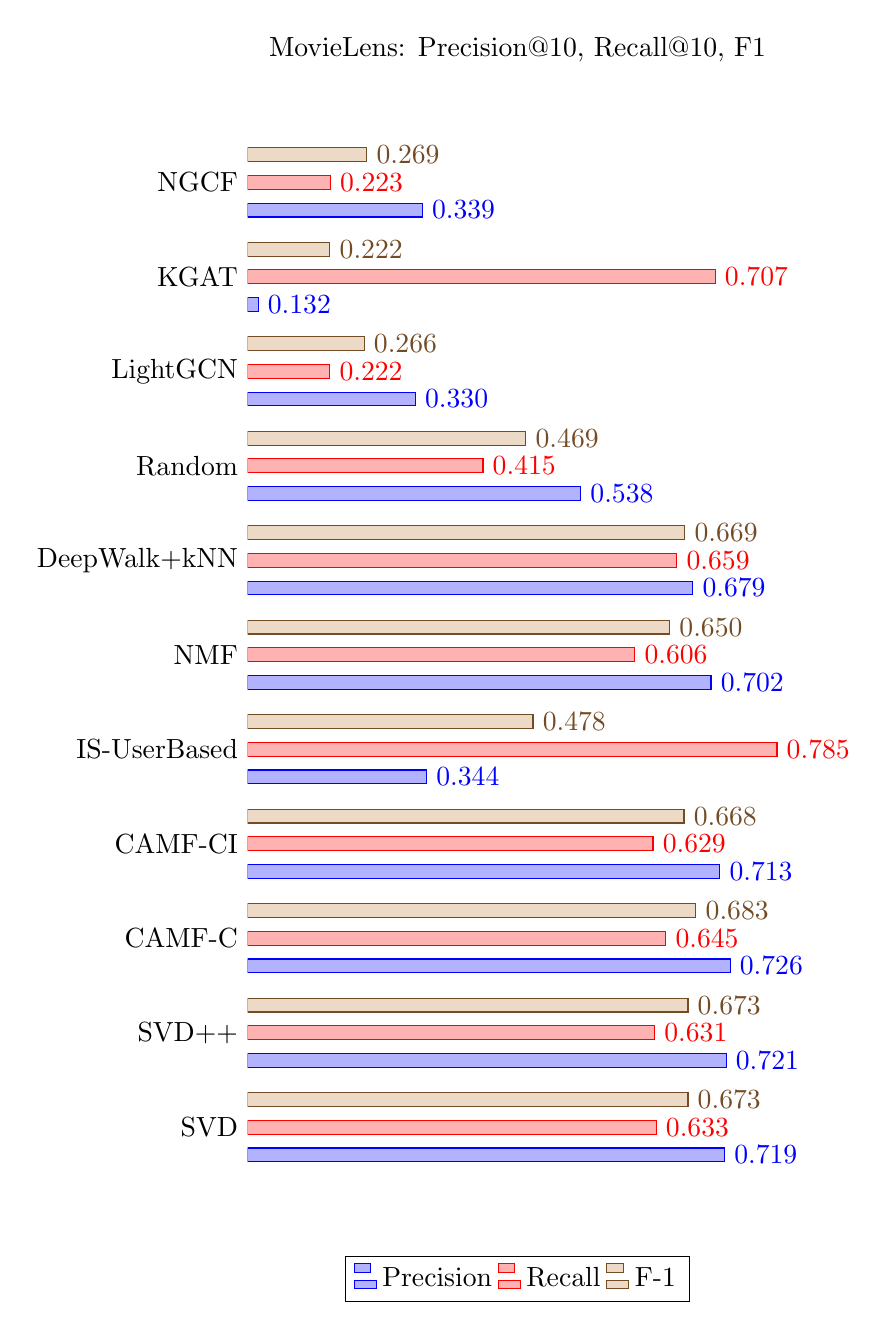
\begin{tikzpicture}
\begin{axis} [
    title    = {MovieLens: Precision@10, Recall@10, F1},
    xbar=5pt,
    /pgf/bar width=5pt,
    y axis line style = { opacity = 0 },
    axis x line       = none,
    tickwidth         = 0pt,
    enlarge x limits  = 0.02,
    ytick=data,
    y=1.2cm,
    nodes near coords={\pgfmathprintnumber[fixed zerofill, precision=3]{\pgfplotspointmeta}},
    legend style={at={(0.5,-0.03)}, anchor=north,legend columns=-1},
    symbolic y coords = {SVD,SVD++,CAMF-C,CAMF-CI,IS-UserBased,NMF,DeepWalk+kNN,Random,LightGCN,KGAT,NGCF},
  ]
\addplot coordinates{(0.719,SVD) (0.721,SVD++) (0.726,CAMF-C) (0.713,CAMF-CI) (0.344,IS-UserBased) (0.702,NMF) (0.679,DeepWalk+kNN) (0.538,Random) (0.3299,LightGCN) (0.1320,KGAT) (0.3386,NGCF)};
\addplot coordinates{(0.633,SVD) (0.631,SVD++) (0.645,CAMF-C) (0.629,CAMF-CI) (0.785,IS-UserBased) (0.606,NMF) (0.659,DeepWalk+kNN) (0.415,Random) (0.2222,LightGCN) (0.7072,KGAT) (0.2228,NGCF)};
\addplot coordinates{(0.673,SVD) (0.673,SVD++) (0.683,CAMF-C) (0.668,CAMF-CI) (0.478,IS-UserBased) (0.650,NMF) (0.669,DeepWalk+kNN) (0.469,Random) (0.265514,LightGCN) (0.222441,KGAT) (0.268757,NGCF)};
\legend{Precision,Recall,F-1}
\end{axis}
\end{tikzpicture}
\label{graph:MLPrecRecF1}
\caption{Precision, recall and F1 results for MovieLens dataset across the investigated methods}
\end{figure}

\begin{figure}[h]
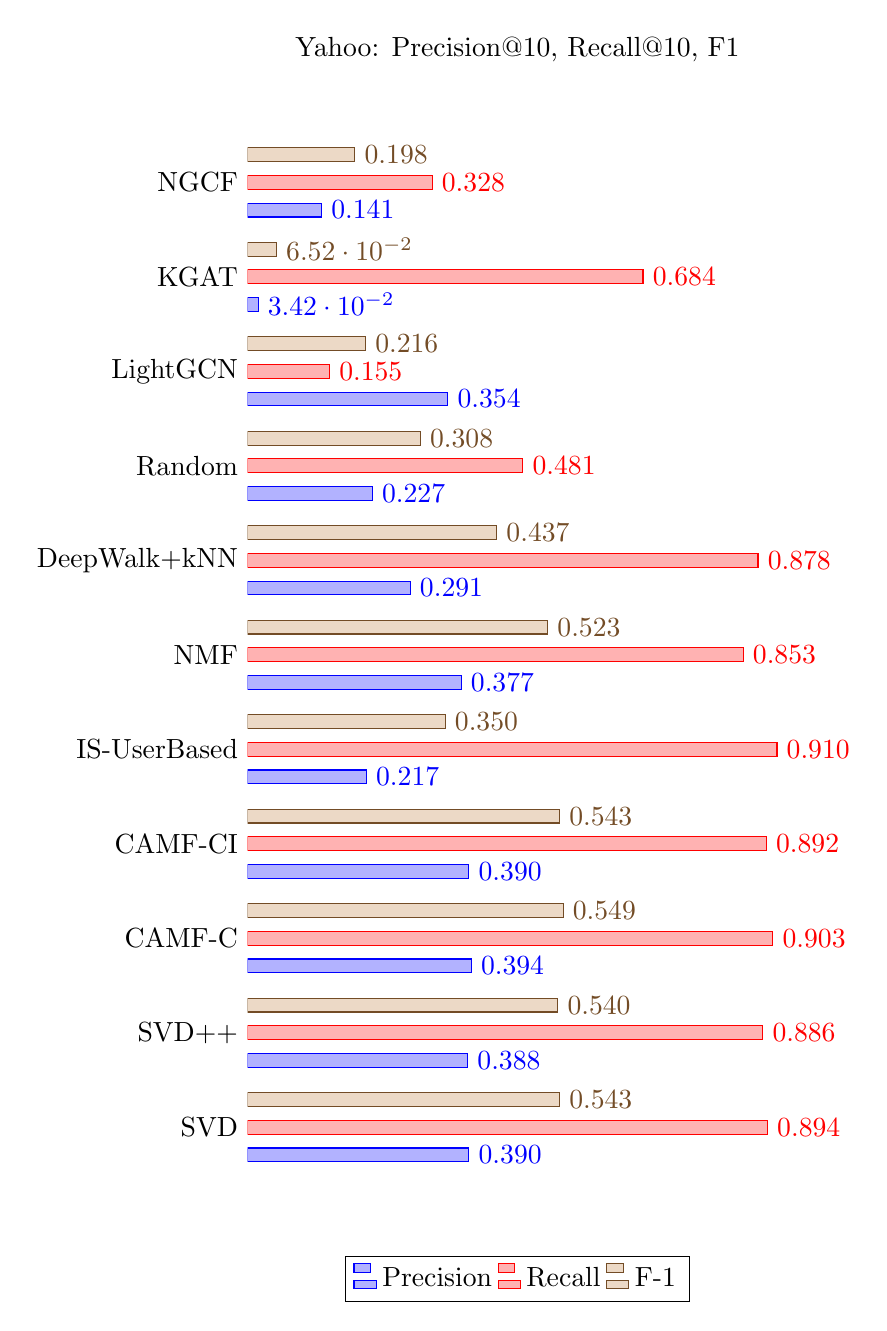
\begin{tikzpicture}
\begin{axis} [
    title    = {Yahoo: Precision@10, Recall@10, F1},
    xbar=5pt,
    /pgf/bar width=5pt,
    y axis line style = { opacity = 0 },
    axis x line       = none,
    tickwidth         = 0pt,
    enlarge x limits  = 0.02,
    ytick=data,
    y=1.2cm,
    nodes near coords={\pgfmathprintnumber[fixed zerofill, precision=3]{\pgfplotspointmeta}},
    legend style={at={(0.5,-0.03)}, anchor=north,legend columns=-1},
    symbolic y coords = {SVD,SVD++,CAMF-C,CAMF-CI,IS-UserBased,NMF,DeepWalk+kNN,Random,LightGCN,KGAT,NGCF},
  ]
\addplot coordinates{(0.390,SVD) (0.388,SVD++) (0.394,CAMF-C) (0.390,CAMF-CI) (0.217,IS-UserBased) (0.377,NMF) (0.291,DeepWalk+kNN) (0.227,Random) (0.3544,LightGCN) (0.0342,KGAT) (0.1414,NGCF)};
\addplot coordinates{(0.894,SVD) (0.886,SVD++) (0.903,CAMF-C) (0.892,CAMF-CI) (0.910,IS-UserBased) (0.853,NMF) (0.878,DeepWalk+kNN) (0.481,Random) (0.1548,LightGCN) (0.6840,KGAT) (0.3280,NGCF)};
\addplot coordinates{(0.543,SVD) (0.540,SVD++) (0.549,CAMF-C) (0.543,CAMF-CI) (0.350,IS-UserBased) (0.523,NMF) (0.437,DeepWalk+kNN) (0.308,Random) (0.2155,LightGCN) (0.0652,KGAT) (0.1976,NGCF)};
\legend{Precision,Recall,F-1}
\end{axis}
\end{tikzpicture}
\label{graph:YahooPrecRecF1}
\caption{Precision, recall and F1 results for Yahoo dataset across the investigated methods}
\end{figure}

\begin{figure}[h]
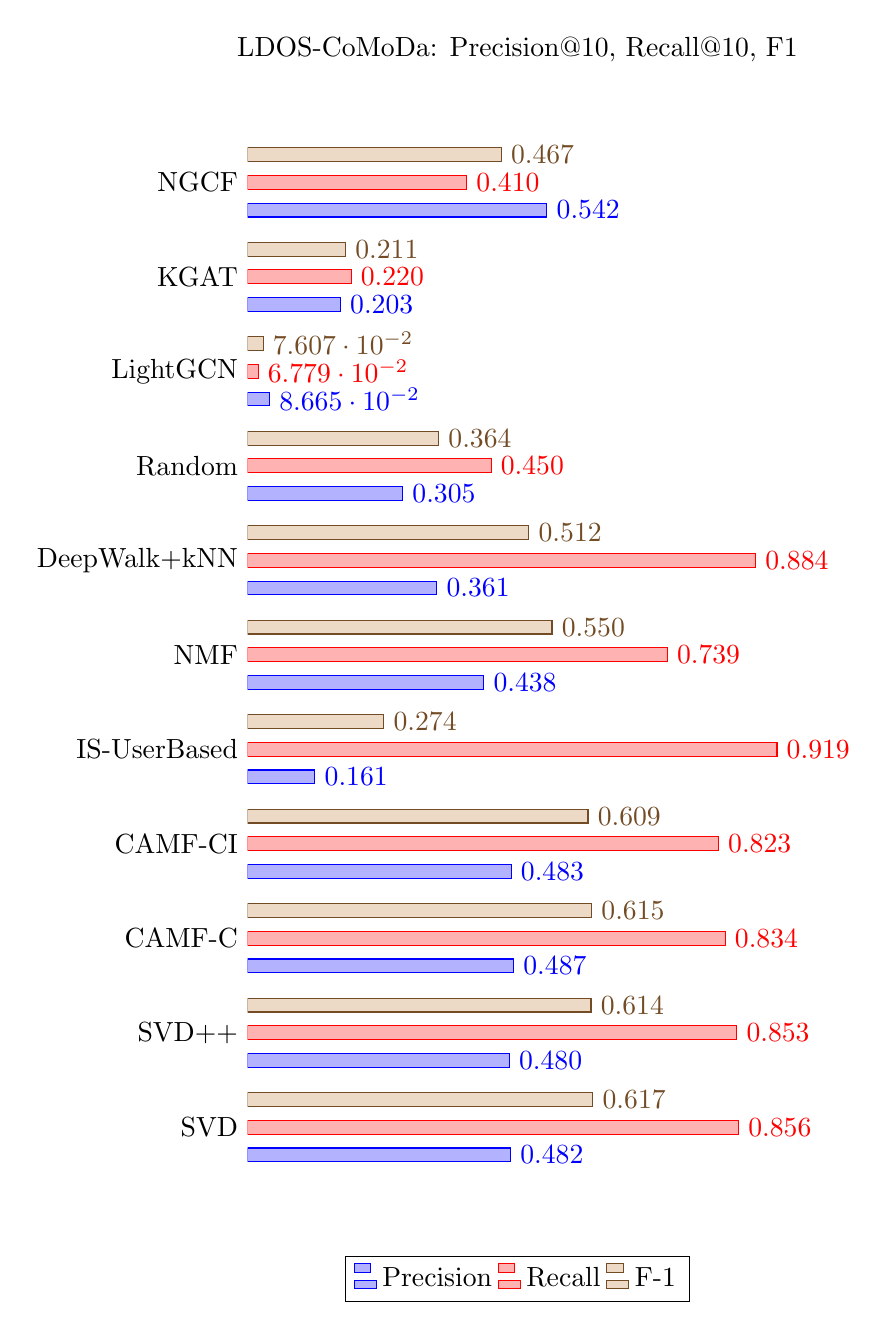
\begin{tikzpicture}
\begin{axis} [
    title    = {LDOS-CoMoDa: Precision@10, Recall@10, F1},
    xbar=5pt,
    /pgf/bar width=5pt,
    y axis line style = { opacity = 0 },
    axis x line       = none,
    tickwidth         = 0pt,
    enlarge x limits  = 0.02,
    ytick=data,
    y=1.2cm,
    nodes near coords={\pgfmathprintnumber[fixed zerofill, precision=3]{\pgfplotspointmeta}},
    legend style={at={(0.5,-0.03)}, anchor=north,legend columns=-1},
    symbolic y coords = {SVD,SVD++,CAMF-C,CAMF-CI,IS-UserBased,NMF,DeepWalk+kNN,Random,LightGCN,KGAT,NGCF},
  ]
\addplot coordinates{(0.482,SVD) (0.480,SVD++) (0.487,CAMF-C) (0.483,CAMF-CI) (0.161,IS-UserBased) (0.438,NMF) (0.361,DeepWalk+kNN) (0.305,Random) (0.08665008,LightGCN) (0.20284,KGAT) (0.5416,NGCF)};
\addplot coordinates{(0.856,SVD) (0.853,SVD++) (0.834,CAMF-C) (0.823,CAMF-CI) (0.919,IS-UserBased) (0.739,NMF) (0.884,DeepWalk+kNN) (0.450,Random) (0.067787792,LightGCN) (0.220396,KGAT) (0.41,NGCF)};
\addplot coordinates{(0.617,SVD) (0.614,SVD++) (0.615,CAMF-C) (0.609,CAMF-CI) (0.274,IS-UserBased) (0.550,NMF) (0.512,DeepWalk+kNN) (0.364,Random) (0.0760671,LightGCN) (0.211254,KGAT) (0.466700,NGCF)};
\legend{Precision,Recall,F-1}
\end{axis}
\end{tikzpicture}
\label{graph:CoMoDaPrecRecF1}
\caption{Precision, recall and F1 results for LDOS-CoMoDa dataset across the investigated methods}
\end{figure}

\begin{figure}[h]
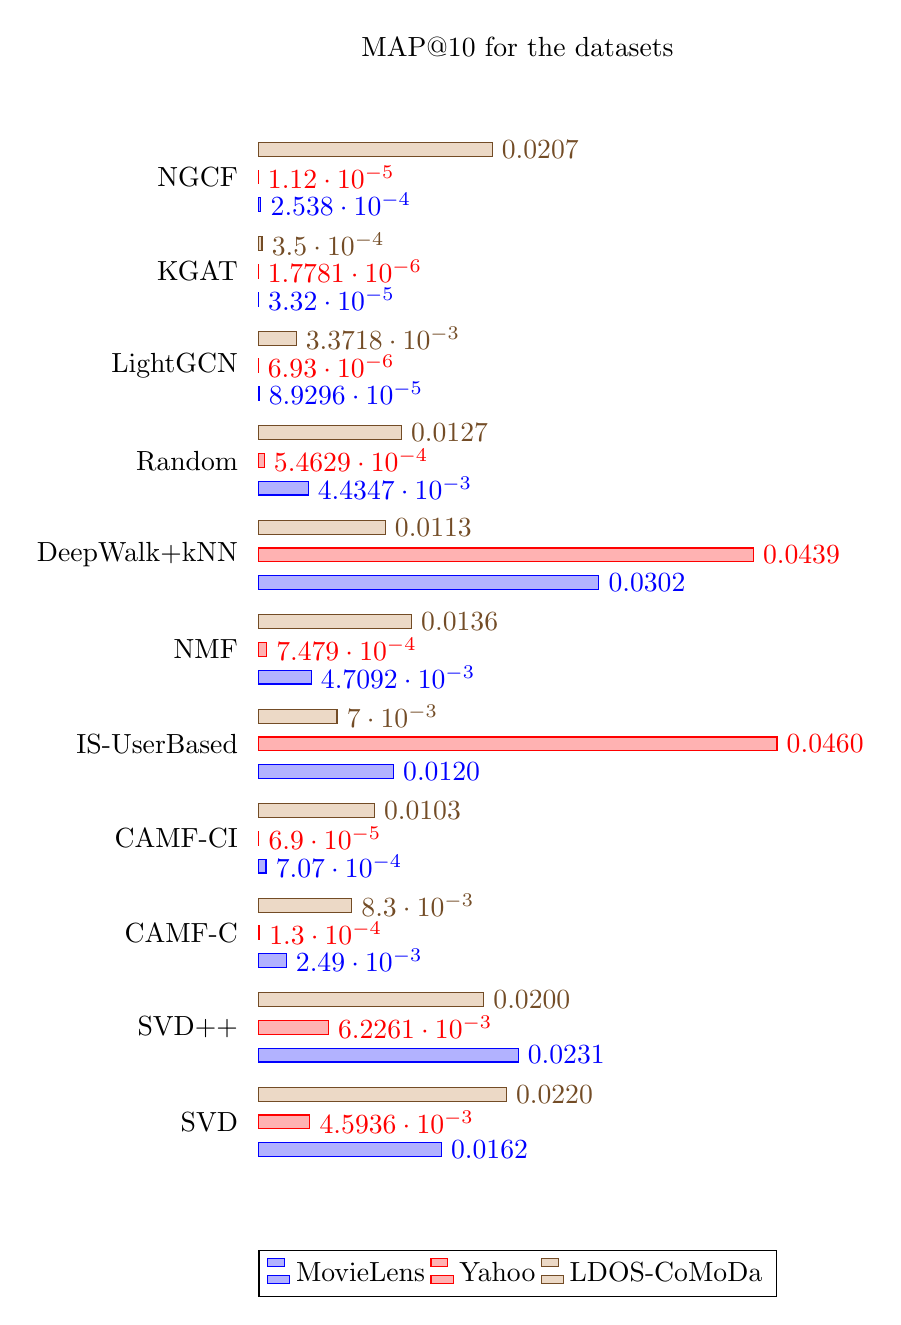
\begin{tikzpicture}
\begin{axis} [
    title    = {MAP@10 for the datasets},
    xbar=5pt,
    /pgf/bar width=5pt,
    y axis line style = { opacity = 0 },
    axis x line       = none,
    tickwidth         = 0pt,
    enlarge x limits  = 0.02,
    ytick=data,
    y=1.2cm,
    nodes near coords={\pgfmathprintnumber[fixed zerofill, precision=4]{\pgfplotspointmeta}},
    legend style={at={(0.5,-0.03)}, anchor=north,legend columns=-1},
    symbolic y coords = {SVD,SVD++,CAMF-C,CAMF-CI,IS-UserBased,NMF,DeepWalk+kNN,Random,LightGCN,KGAT,NGCF},
  ]
\addplot coordinates{(0.0162465951248284,SVD) (0.0230514217391177,SVD++) (0.00249,CAMF-C) (0.000707,CAMF-CI) (0.0120,IS-UserBased) (0.00470921880091866,NMF) (0.0302,DeepWalk+kNN) (0.00443467504522534,Random) (0.0000892961875081354,LightGCN) (0.0000332,KGAT) (0.0002538,NGCF)}; % MovieLens
\addplot coordinates{(0.00459364446058646,SVD) (0.00622607894470324,SVD++) (0.00013,CAMF-C) (0.000069,CAMF-CI) (0.046,IS-UserBased) (0.000747900814877045,NMF) (0.0439,DeepWalk+kNN) (0.000546288347257189,Random) (0.00000693,LightGCN) (0.0000017781423399345,KGAT) (0.0000112,NGCF)}; % Yahoo
\addplot coordinates{(0.022,SVD) (0.02,SVD++) (0.0083,CAMF-C) (0.0103,CAMF-CI) (0.007,IS-UserBased) (0.0136,NMF) (0.01127,DeepWalk+kNN) (0.0126990696917064,Random) (0.00337181254,LightGCN) (0.00035,KGAT) (0.020748,NGCF)}; % CoMoDa
\legend{MovieLens,Yahoo,LDOS-CoMoDa}
\end{axis}
\end{tikzpicture}
\label{graph:MAP10}
\caption{MAP@10 results for the dataset across the investigated methods}
\end{figure}

\begin{figure}[h]
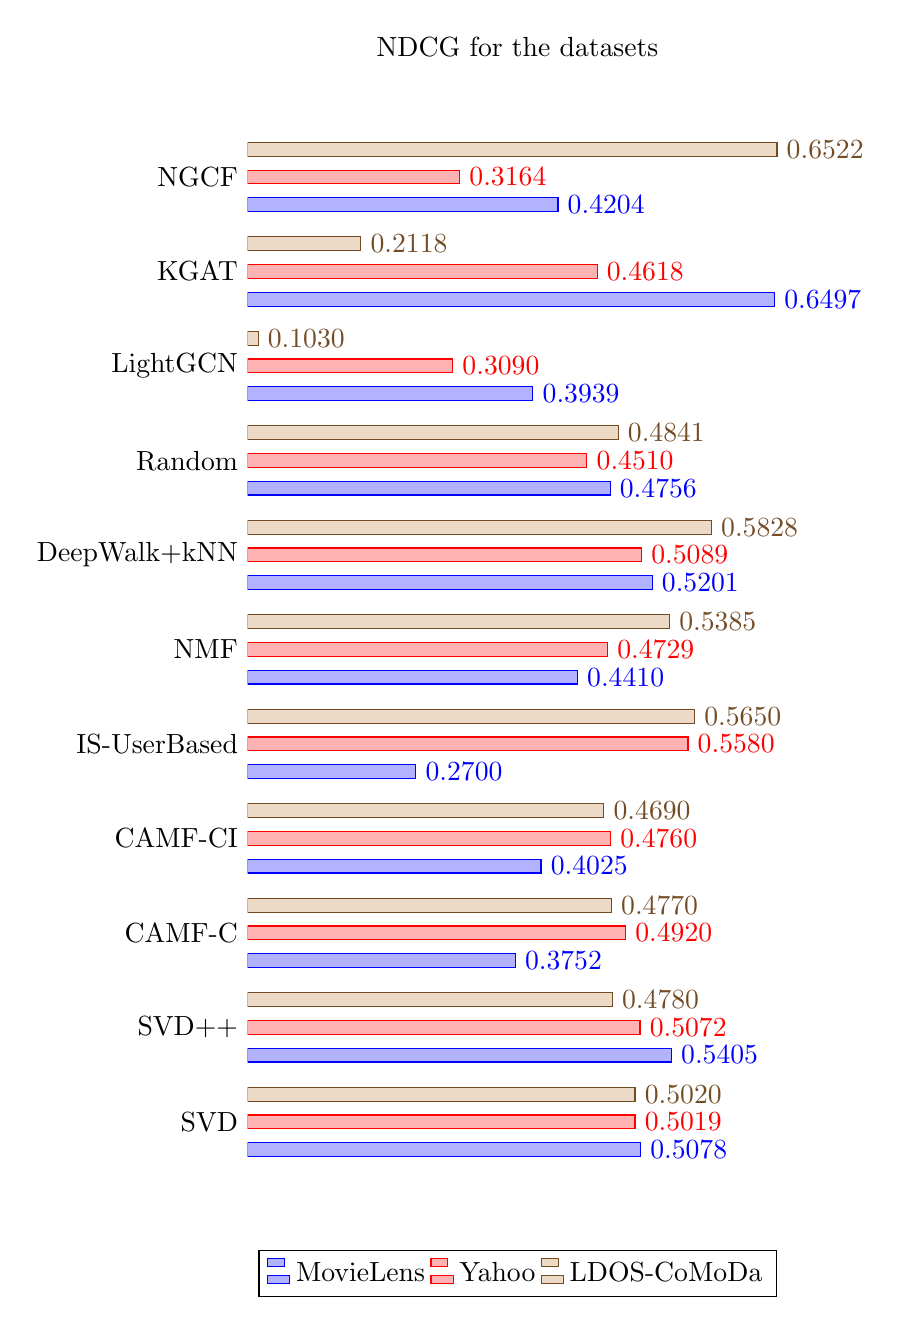
\begin{tikzpicture}
\begin{axis} [
    title    = {NDCG for the datasets},
    xbar=5pt,
    /pgf/bar width=5pt,
    y axis line style = { opacity = 0 },
    axis x line       = none,
    tickwidth         = 0pt,
    enlarge x limits  = 0.02,
    ytick=data,
    y=1.2cm,
    nodes near coords={\pgfmathprintnumber[fixed zerofill, precision=4]{\pgfplotspointmeta}},
    legend style={at={(0.5,-0.03)}, anchor=north,legend columns=-1},
    symbolic y coords = {SVD,SVD++,CAMF-C,CAMF-CI,IS-UserBased,NMF,DeepWalk+kNN,Random,LightGCN,KGAT,NGCF},
  ]
\addplot coordinates{(0.507788476243958,SVD) (0.540462250066491,SVD++) (0.3752,CAMF-C) (0.4025,CAMF-CI) (0.270,IS-UserBased) (0.441025641977599,NMF) (0.5201,DeepWalk+kNN) (0.475627993916583,Random) (0.3939,LightGCN) (0.6497,KGAT) (0.4204,NGCF)}; % MovieLens
\addplot coordinates{(0.501928001717915,SVD) (0.507223962441533,SVD++) (0.492,CAMF-C) (0.476,CAMF-CI) (0.558,IS-UserBased) (0.472880077638768,NMF) (0.5089,DeepWalk+kNN) (0.451040991988228,Random) (0.3090,LightGCN) (0.4618,KGAT) (0.3164,NGCF)}; % Yahoo
\addplot coordinates{(0.502,SVD) (0.478,SVD++) (0.477,CAMF-C) (0.469,CAMF-CI) (0.565,IS-UserBased) (0.5385,NMF) (0.5828,DeepWalk+kNN) (0.484100128099788,Random) (0.103,LightGCN) (0.21176,KGAT) (0.6522,NGCF) }; % CoMoDa
\legend{MovieLens,Yahoo,LDOS-CoMoDa}
\end{axis}
\end{tikzpicture}
\label{graph:NDCG10}
\caption{NDCG@10 results for the dataset across the investigated methods}
\end{figure}